\begin{mainquestion}{sourcefollower}{Source Follower Measurement}

\begin{center}
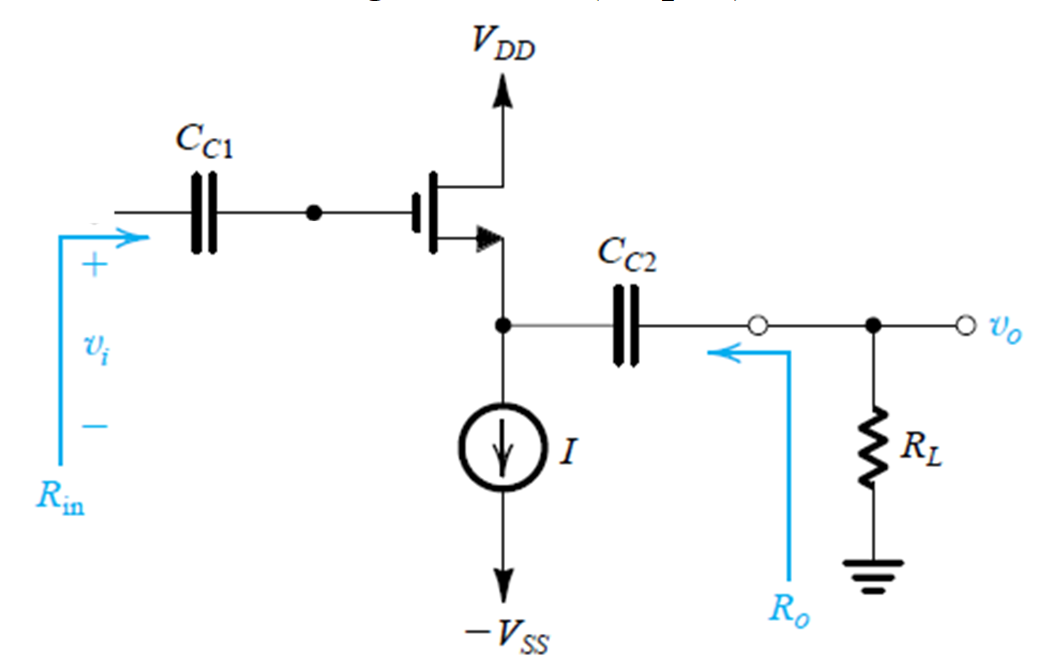
\includegraphics[width=4.5in]{questionbank/amplifiers/source_follower/v0/image7.png}
\end{center}

A source-follower circuit is shown below. With $R_L$ removed, the open-circuit voltage gain $A_{vo} = \frac{v_o}{v_i}$ is carefully measured and found to be 0.88. Then, when $R_L$  is connected and its value is varied, we find the gain is halved at $R_L = \qty{2}{\kilo\ohm}$. If the amplifier remained linear during the measurement, what are the values of $g_m$ and $r_o$?

\begin{partquestion}{gm}{Find $g_m$}
\begin{answer}

\begin{kaitlyn}
    \noindent\fbox{%
    \begin{minipage}{\dimexpr\textwidth-2\fboxsep-2\fboxrule\relax}   

        \textbf{How to approach this problem:} Use loading to determine the amplifier’s $R_o$, then zoom into the MOSFET small-signal model to determine what $g_m$ and $r_o$ produce that $R_o$

\end{minipage}%
}
\end{kaitlyn}
The open-circuit gain of the source follower (common-drain) stage without a load is:

\[
A_{vo} = \frac{v_{o}}{v_{i}} = \frac{g_{m} r_{o}}{1 + g_{m} r_{o}} = 0.88.
\]

With a load, the total gain is a voltage divider:

\[
A_{v} = A_{vo} \frac{R_{L}}{R_{L} + R_{o}}.
\]

If this gain is halved by connecting $R_{L} = \qty{2}{\kilo\ohm}$, then $R_{o} = \qty{2}{\kilo\ohm}$.

Since the resistance of the common drain output is $R_{o} = \frac{r_{o}}{1 + g_{m} r_{o}}$, taking the ratio of the first and third equations gives:

\[
g_{m} = \frac{A_{vo}}{R_{o}} = \frac{0.88}{2000} = 0.44\ \text{mS}.
\]
\end{answer}
\end{partquestion}

\begin{partquestion}{ro}{Find $\mathbf{r}_{\mathbf{o}}$}
\begin{answer}
Use the relationship between $R_{o}$, $g_{m}$, and $r_{o}$:

\[
R_{o} = \frac{r_{o}}{1 + g_{m} r_{o}} = \qty{2}{\kilo\ohm}.
\]

Solve for $r_{o}$ using the measured values:

\begin{align*}
    r_o &= \frac{R_o}{1 - R_o g_m} \\
    &= \frac{2000}{1 - 2000(0.00044)} = \qty{16.7}{\kilo\ohm}
\end{align*}

We can safely round this to \qty{17}{\kilo\ohm} to appease the universe. 

\end{answer}
\end{partquestion}

\end{mainquestion}
